
\begin{figure}[h]
  \centering
{
\begin{tabular}{cc}
      \subfloat[Data block size = 64 KBytes]{
        \scalebox{0.39}{
          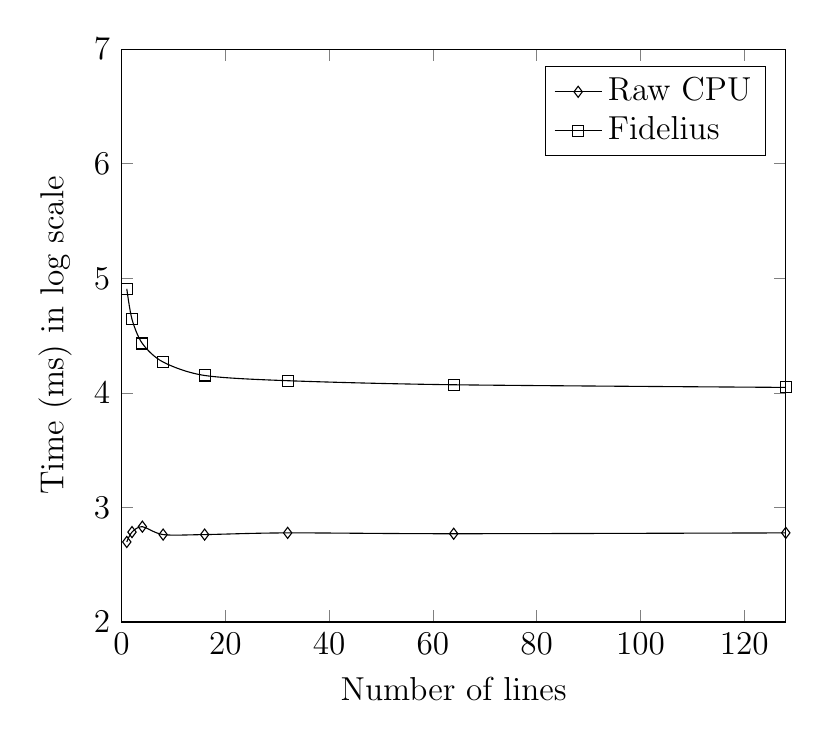
\begin{tikzpicture}
            
\large
\pgfplotsset{
    scale only axis,
    xmin=0, xmax=128,
    compat=newest,
    legend pos=north east,
}

\begin{axis}[
  %axis y line*=left,
  %scaled y ticks=base 10:2,
  %ymin=0, ymax=0.0004,
  %ymin=0, ymax=0.008,
  ymin=2, ymax=7,
  xlabel=Number of lines,
  %width=0.4\textwidth,
  %height=0.6\textwidth,
  ylabel=Time (ms) in log scale,
]

\addplot[smooth,mark=diamond]
  coordinates{
    (1,2.6990) %log10(500)
    (2,2.7853) %log10(610)
    (4,2.8325) %log10(680)
    (8,2.7634) %log10(580)
    (16,2.7634) %log10(580)
    (32,2.7782) %log10(600)
    (64,2.7709) %log10(590)
    (128,2.7782) %log10(600)
}; \label{plot_raw}

\addplot[smooth,mark=square]
  coordinates{
    (1,4.9085) %log10(81000)
    (2,4.6435) %log10(44000)
    (4,4.4314) %log10(27000)
    (8,4.2695) %log10(18600)
    (16,4.1523) %log10(14200)
    (32,4.1065) %log10(12780)
    (64,4.0711) %log10(11780)
    (128,4.0481) %log10(11170)
  }; \label{plot_fid}



  \addlegendimage{/pgfplots/refstyle=plot_raw}\addlegendentry[right]{Raw CPU}
  \addlegendimage{/pgfplots/refstyle=plot_fid}\addlegendentry[right]{Fidelius}

\end{axis}
          \end{tikzpicture}
        }
      } &
      \subfloat[Data block size = 256 KBytes]{
        \scalebox{0.39}{
          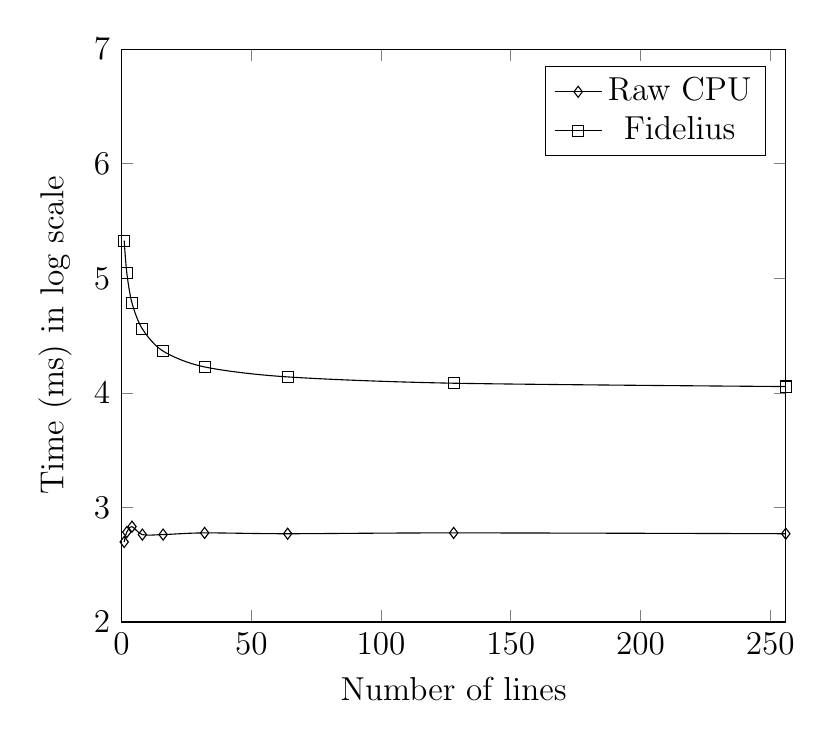
\begin{tikzpicture}
            
\large
\pgfplotsset{
    scale only axis,
    xmin=0, xmax=256,
    compat=newest,
    legend pos=north east,
}

\begin{axis}[
  %axis y line*=left,
  %scaled y ticks=base 10:2,
  %ymin=0, ymax=0.0004,
  %ymin=0, ymax=0.008,
  ymin=2, ymax=7,
  xlabel=Number of lines,
  %width=0.4\textwidth,
  %height=0.6\textwidth,
  ylabel=Time (ms) in log scale,
]
1	0.5	    213
2	0.61	111.78
4	0.68	61.04
8	0.58	36.2
16	0.58	23.16
32	0.6	    16.85
64	0.59	13.79
128	0.6	    12.15
256	0.59	11.36
\addplot[smooth,mark=diamond]
  coordinates{
    (1,2.6990) %log10(500)
    (2,2.7853) %log10(610)
    (4,2.8325) %log10(680)
    (8,2.7634) %log10(580)
    (16,2.7634) %log10(580)
    (32,2.7782) %log10(600)
    (64,2.7709) %log10(590)
    (128,2.7782) %log10(600)
    (256, 2.7709) %log10(590)
}; \addlegendentry{Raw CPU}

\addplot[smooth,mark=square]
  coordinates{
    (1,5.3284) %log10(213000)
    (2,5.0484) %log10(111780)
    (4,4.7856) %log10(61040)
    (8,4.5587) %log10(36200)
    (16,4.3647) %log10(23160)
    (32,4.2266) %log10(16850)
    (64,4.1396) %log10(13790)
    (128,4.0846) %log10(12150)
    (256,4.0554) %log10(11360)
  }; \addlegendentry{Fidelius}

\end{axis}
          \end{tikzpicture}
        }
      }    \\
\end{tabular}
  }
  \caption{\small Time Consumption of I/O-Intensive Task.}
  \label{fig:io_intensive}
\end{figure}
